\documentclass[journal,12pt,twocolumn]{IEEEtran}
\usepackage{graphicx}
\usepackage{amsmath}
\usepackage{amssymb}
\usepackage{float}
\usepackage{caption}
\providecommand{\brak}[1]{\ensuremath{\left(#1\right)}}
\newcommand{\question}{\noindent\large \textbf{Question: }}
\newcommand{\solution}{\noindent\large \textbf{Solution: }}
\begin{document}
\title{ASSIGNMENT 2}
\author{AKHILA, CS21BTECH11031}

\maketitle
\question
If $x=tan\brak{logy}$, prove that 
\begin{equation*}
    \brak{1+x^2}\frac{d^2y}{d x^2}+\brak{2x-1}\frac{dy}{dx}=0
\end{equation*}
\solution
Given, $x=tan\brak{logy}$
\begin{align}
    &\implies \tan^{-1} x =logy\\
    &\implies y= e^{\tan^{-1}x}\label{eq1}
\end{align}
Differentiating on both sides with respect to x..
\begin{align}
     &\implies\frac{dy}{dx}= \frac{d}{dx}\brak{e^{\tan^{-1} x}}\\
     &\implies\frac{dy}{dx}=\brak{e^{\tan^{-1} x}}\frac{d}{dx}\brak{\tan^{-1} x}\\
     &\implies\frac{dy}{dx}=\brak{e^{\tan^{-1} x}}\brak{\frac{1}{1+x^2}}\\
     &\implies\frac{dy}{dx}=\frac{ e^{\tan^{-1} x}}{1+x^2}
\end{align}
From \eqref{eq1}...
\begin{equation}
\label{eq2}
     \therefore \frac{dy}{dx} = \frac{y}{1+x^2} 
\end{equation}
Again differentiating on both sides with respect to x..
\begin{align}
    \implies\frac{d^2y}{dx^2} =\frac{d}{dx}\brak{\frac{y}{1+x^2}}\\
    =\frac{d}{dx}\brak{\frac{1}{1+x^2}}y+\frac{1}{1+x^2}\frac{dy}{dx} \\
    =\frac{-1(2x)}{\brak{1+x^2}^2} \brak{y}+\frac{1}{1+x^2}\frac{dy}{dx} \\
    =\frac{-2x}{(1+x^2)}\frac{y}{(1+x^2)} +\frac{1}{1+x^2}\frac{dy}{dx} 
\end{align}
From \eqref{eq2}...
\begin{align}
    &\implies \frac{d^2y}{dx^2}=\frac{-2x}{\brak{1+x^2}}\frac{dy}{dx} +\frac{1}{\brak{1+x^2}}\frac{dy}{dx} \\
    &\implies \brak{1+x^2}\frac{d^2y}{dx^2}=\frac{dy}{dx}\brak{1-2x}\\
    &\implies \brak{1+x^2}\frac{d^2y}{dx^2}=-\frac{dy}{dx}\brak{2x-1}\\
    &\therefore \brak{1+x^2}\frac{d^2y}{dx^2}+\frac{dy}{dx}\brak{2x-1}=0
\end{align}
     Hence proved.
\begin{figure}[H]
    \centering
    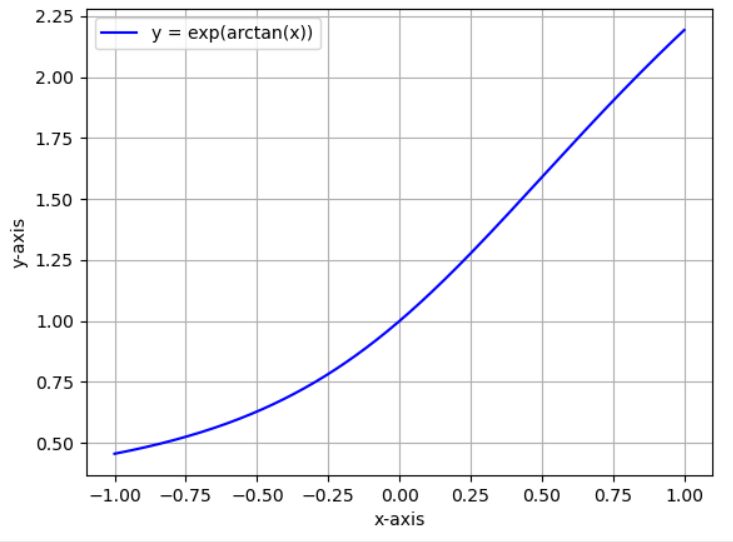
\includegraphics[width=\columnwidth]{plot3.png}
    \captionsetup{justification=centering,margin=1cm}
    \caption{Graph of $y= e^{\tan^{-1}x}$}
    \label{fig:plot3}
\end{figure}
\end{document}
